\documentclass[11pt]{article}
\usepackage[utf8]{inputenc}
\usepackage{amsmath,amsthm,amsfonts,amssymb,amscd}
\usepackage{multirow,booktabs}
\usepackage[table]{xcolor}
\usepackage{fullpage}
\usepackage{lastpage}
\usepackage{enumitem}
\usepackage{fancyhdr}
\usepackage{mathrsfs}
\usepackage{wrapfig}
\usepackage{setspace}
\usepackage{calc}
\usepackage{multicol}
\usepackage{cancel}
\usepackage[retainorgcmds]{IEEEtrantools}
\usepackage[margin=1in, headsep=0.25in]{geometry}
\usepackage{empheq}
\usepackage{framed}
\usepackage[most]{tcolorbox}
\usepackage{soul}
\usepackage{algorithm}
\usepackage{algpseudocode}
\usepackage[style=ieee, backend=biber]{biblatex}
\addbibresource{references.bib}
\usepackage{tikz}
\usetikzlibrary{decorations.pathmorphing,patterns,arrows.meta,calc,positioning}

% --- MNNW palette -------------------------------------------------------
\definecolor{mnnwInk}     {HTML}{0A0A0A}
\definecolor{mnnwSignal}  {HTML}{0A84FF}
\definecolor{mnnwHair}    {HTML}{C9C9C9}
\definecolor{mnnwMute}    {HTML}{6F6F6F}
\definecolor{reticleFill} {HTML}{DCE6F7}  % light blue (reticle, j=1)
\definecolor{reticleEdge} {HTML}{4F6F9F}
\definecolor{reticleFlex} {HTML}{EEF3FB}  % flex couplings, lighter
\definecolor{waferFill}   {HTML}{F5DCDC}  % light red (wafer, j=3)
\definecolor{waferEdge}   {HTML}{9F4F4F}
\definecolor{waferFlex}   {HTML}{FBEEEE}
\definecolor{opticsFill}  {HTML}{E7DCF5}  % light purple (optics, j=2)
\definecolor{opticsEdge}  {HTML}{6F4F9F}
\definecolor{opticsFlex}  {HTML}{F3EEFB}
\definecolor{frameFill}   {HTML}{D9E8D2}  % light green (frames F1,F2)
\definecolor{frameEdge}   {HTML}{4F7F3F}
\definecolor{lensFill}    {HTML}{EEEEEE}

% --- Spring/damper pics --------------------------------------------------
\tikzset{
  hdamper/.pic={
    \draw[line width=0.5pt, mnnwInk] (-0.45,0)            -- (-0.18,0);
    \draw[line width=0.5pt, mnnwInk] (-0.18,-0.11) rectangle (0.18,0.11);
    \draw[line width=0.5pt, mnnwInk] (0,-0.11)            -- (0,0.11);
    \draw[line width=0.5pt, mnnwInk] (0.18,0)             -- (0.45,0);
  },
  vdamper/.pic={
    \draw[line width=0.5pt, mnnwInk] (0,-0.45)            -- (0,-0.18);
    \draw[line width=0.5pt, mnnwInk] (-0.11,-0.18) rectangle (0.11,0.18);
    \draw[line width=0.5pt, mnnwInk] (-0.11,0)            -- (0.11,0);
    \draw[line width=0.5pt, mnnwInk] (0,0.18)             -- (0,0.45);
  },
}

\colorlet{shadecolor}{orange!15}
\parindent 0in
\parskip 12pt
\geometry{margin=1in, headsep=0.25in}
\theoremstyle{definition}
\newtheorem{defn}{Definition}
\newtheorem{reg}{Rule}
\newtheorem{exer}{Exercise}
\newtheorem{note}{Note}
\begin{document}
\setcounter{section}{8}
\title{Theoretical Framework}

\thispagestyle{empty}

\begin{center}
{\LARGE \bf Theoretical Framework}\\
%{\large Physics 300}\\
%Fall 2016
\end{center}

\section{Introduction}

The history of modern electronics is inseparable from the history of lithography. Since the independent invention of the integrated circuit (IC) by Jack Kilby at Texas Instruments and Robert Noyce at Fairchild Semiconductor in 1958, Moore's Law has governed the relentless progression of the semiconductor industry: the density of components on a chip doubles approximately every two years \cite{Schmidt2012_UltraPrecision}. This exponential trajectory has translated into dramatic reductions in cost alongside equally dramatic increases in performance. The price of one gigabyte of NAND flash memory, for instance, fell from over \$1000 at the start of this millennium to below \$0.30 by the mid-2010s \cite{Butler2011_PositionControl}, while the minimum transistor feature size has shrunk from hundreds of nanometres to just a few tens of nanometres. The engine of this revolution is \textit{photolithography} — the process by which the intricate patterns of a transistor, a wire, or a memory cell are projected onto a silicon wafer with nanometre-scale fidelity.

The fabrication of a modern IC consists of up to 30 sequential process cycles, each defining one distinct layer of the device \cite{Schmidt2012_UltraPrecision}. A monocrystalline silicon wafer — a thin disc of up to 300\,mm in diameter — serves as the substrate throughout this process. Each cycle begins with a chemical pre-treatment, such as the thermal growth of a thin oxide film for electrical isolation. A photosensitive material called \textit{resist} is then deposited onto the wafer surface. An optical exposure system projects the pattern for the current layer — defined in a chromium film on a transparent quartz plate known as the \textit{reticle}, or \textit{photo-mask} — onto the resist. After development, the regions that received light are selectively dissolved (in the case of a positive resist), exposing the underlying material. This material then undergoes one of several process steps. \textit{Plasma etching} selectively removes oxide or semiconductor material to define trenches and isolation regions. \textit{Ion implantation} locally modifies the electrical properties of the silicon to form transistor junctions and doped wells. \textit{Physical or chemical vapour deposition} lays down thin films of conductive metal — typically tungsten or copper — to form the interconnecting wiring that links the millions of functional elements stacked across all layers. After processing, the remaining resist is stripped and the cycle repeats for the next layer, until all layers are complete and the wafer is diced and packaged.

In the earliest days of the industry, the reticle was brought into direct physical contact with the resist-coated wafer during exposure — a technique known as \textit{contact lithography}. While simple, this approach had two fundamental shortcomings. First, repeated physical contact progressively contaminated and damaged the delicate reticle pattern, necessitating its costly and time-consuming replacement. Second, a 1:1 projection offers no optical resolution advantage: any defect present on the reticle is transferred at full size onto the wafer. These limitations motivated a transition to \textit{projection optical lithography}, in which a reduction lens images the reticle pattern onto the wafer from a safe working distance. The projection lens introduces a demagnification factor of four, meaning that features on the reticle are printed four times smaller on the wafer, immediately relaxing the demands on reticle fabrication. The minimum printable feature size, known as the \textit{critical dimension} (CD), is governed by \cite{Schmidt2012_UltraPrecision}:
\begin{equation}
    \mathrm{CD} = k\,\frac{\lambda}{\mathrm{NA}},
    \label{eq:rayleigh}
\end{equation}
where $\lambda$ is the illumination wavelength, $\mathrm{NA}$ is the numerical aperture of the projection lens, and $k$ is a process-dependent factor. Reducing CD requires a shorter wavelength, a higher NA, and process improvements that lower $k$. This relation has driven a continuous push toward shorter wavelengths — from mercury arc-lamp sources at 436\,nm and 365\,nm, through excimer lasers at 248\,nm and 193\,nm, to the extreme ultraviolet (EUV) sources at 13.5\,nm now entering production.

Achieving a high numerical aperture, however, comes with a practical constraint. Since $\mathrm{NA} = n\sin\vartheta$, where $\vartheta$ is the half-angle of the marginal ray accepted by the lens, attaining values of NA close to one in air requires the lens to subtend a very wide solid angle. Constructing a lens element that simultaneously covers the full area of a 300\,mm wafer at high NA would require an optical element of impractical size and cost \cite{Schmidt2012_UltraPrecision}. The industry's solution was to accept a smaller \textit{exposure field} — typically $26 \times 32$\,mm, corresponding to a single IC die — and expose the wafer in successive steps: after each die is exposed, the wafer stage repositions the wafer to the next die location and the exposure is repeated. This architecture defines the \textit{wafer stepper}. In a stepper, each die is illuminated in a single, instantaneous full-field flash, with the stage brought to a complete stop before exposure commences.

While the stepper represented a decisive step forward, exposing an entire die simultaneously subjects the full field to any non-uniformities in the illumination intensity or lens aberrations. The \textit{scanner} addresses this by replacing the full-field flash with a \textit{scanning exposure}: the illumination system reveals only a narrow rectangular slit of the reticle, and the reticle stage sweeps the mask through this slit while the wafer stage moves synchronously in the opposite direction, maintaining the 4:1 demagnification relationship throughout \cite{Butler2011_PositionControl, Schmidt2012_UltraPrecision}. Because the reticle moves at four times the speed of the wafer, it traverses the full reticle pattern in the same time that the wafer moves one die height. This scanning motion offers significant advantages over full-field exposure: it averages out illumination dose non-uniformities across the exposure field, improves imaging uniformity at the field edges, and allows the use of a physically larger reticle that is easier to write with electron-beam pattern generators. After each die is scanned, the wafer is stepped to the next die position and the scan repeats, defining the \textit{step-and-scan} cycle that gives modern lithographic tools their name. A throughput of over 175 wafers per hour — corresponding to less than 0.2\,s of exposure time per die — is not uncommon in state-of-the-art tools \cite{Butler2011_PositionControl}.

A critical consequence of the multi-layer nature of IC fabrication is the requirement that each new layer be positioned with nanometre-level accuracy relative to all preceding layers — a specification known as \textit{overlay}. The functional layers of a chip are interconnected by millions of tiny conductive pillars called \textit{vias}; a misregistration between consecutive layers of even a few nanometres can misalign a via, break an intended connection, or create an unintended short circuit, rendering the IC defective \cite{Schmidt2012_UltraPrecision}. Overlay requirements scale roughly in proportion with the CD and currently sit below 4\,nm for leading-edge nodes. Overlay is therefore one of the primary technology drivers in scanner design, and it is governed directly by the positioning accuracy of the wafer and reticle stages during the scanning exposure.

The commercial performance of a scanner is ultimately measured in wafers per hour (WPH), since a machine whose capital cost can exceed \$150 million must generate revenue continuously. Although the exposure time per die is fixed by the optics and the process, the time spent stepping and \textit{settling} — the interval between the end of a step motion and the moment the stage has damped its residual vibrations to within the nanometre-level positioning specification — represents a significant and controllable fraction of the total cycle time \cite{Butler2011_PositionControl}, which places the allowable settle time below 10\,ms. Every millisecond saved in settling directly translates into more dies exposed per hour and thus more chips delivered per unit time, with a lower cost per chip. Reducing settling time is therefore a central objective in scanner control engineering.

It is worth noting that, while EUV lithography at 13.5\,nm has entered high-volume production for leading-edge nodes below 10\,nm, deep ultraviolet (DUV) optical lithography at 193\,nm remains the dominant technology for \textit{mature nodes} — technology generations at 28\,nm and above. Mature-node chips are the backbone of automotive electronics, industrial controllers, power management devices, analogue circuits, and the vast majority of consumer electronics. The aggregate volume of wafers produced at mature nodes substantially exceeds that at leading-edge nodes, and is projected to remain so for the foreseeable future. Throughput improvements in DUV step-and-scan tools therefore continue to have a large global impact.

The key lever for reducing settling time — and thus for increasing scanner throughput — is the generation of \textit{reference trajectories}: motion profiles that command the stage from its current position to the next scanning start-point with minimal excitation of mechanical resonances and the shortest possible residual settling tail. A well-designed trajectory limits the energy injected into the structural eigenmodes of the machine, reduces induced vibrations in the sensitive metrology and optical systems, and enables the stage to reach nanometre-level positioning accuracy well within the allocated window. The design of such trajectories is a problem of direct industrial relevance, and forms the central subject of this work.

% --- Spring/damper pics --------------------------------------------------
% Long-form damper: cylinder body + protruding piston rod, total length 2L.
% Cylinder anchors at left, piston rod exits to the right.
%   #1 = full length (cm).  Piston-rod length is half of total.
\tikzset{
  vdamper/.pic={
    \draw[line width=0.5pt, mnnwInk] (0,-0.45)            -- (0,-0.18);
    \draw[line width=0.5pt, mnnwInk] (-0.11,-0.18) rectangle (0.11,0.18);
    \draw[line width=0.5pt, mnnwInk] (-0.11,0)            -- (0.11,0);
    \draw[line width=0.5pt, mnnwInk] (0,0.18)             -- (0,0.45);
  },
}
% Long horizontal damper between (xa, y) and (xb, y).
% Cylinder is the LEFT 60%, piston rod the RIGHT 40%.
\newcommand{\hdamperLong}[3]{%
  \pgfmathsetmacro{\xa}{#1}\pgfmathsetmacro{\xb}{#2}\pgfmathsetmacro{\yy}{#3}
  \pgfmathsetmacro{\Lcyl}{(\xb-\xa)*0.55}
  \pgfmathsetmacro{\xcylR}{\xa+\Lcyl}
  \pgfmathsetmacro{\xpisR}{\xb}
  % cylinder body (open on the right end)
  \draw[line width=0.5pt, mnnwInk] (\xa,\yy-0.13) -- (\xa,\yy+0.13);% closed left wall
  \draw[line width=0.5pt, mnnwInk] (\xa,\yy+0.13) -- (\xcylR,\yy+0.13);
  \draw[line width=0.5pt, mnnwInk] (\xa,\yy-0.13) -- (\xcylR,\yy-0.13);
  % piston disc inside cylinder (about 70% along)
  \pgfmathsetmacro{\xpiston}{\xa+\Lcyl*0.70}
  \draw[line width=0.5pt, mnnwInk] (\xpiston,\yy-0.11) -- (\xpiston,\yy+0.11);
  % piston rod from disc to right anchor
  \draw[line width=0.5pt, mnnwInk] (\xpiston,\yy) -- (\xpisR,\yy);
}
% Long vertical damper between (x, ya) and (x, yb).
% Cylinder is the BOTTOM 60%, piston rod the TOP 40%.
\newcommand{\vdamperLong}[3]{%
  \pgfmathsetmacro{\xx}{#1}\pgfmathsetmacro{\ya}{#2}\pgfmathsetmacro{\yb}{#3}
  \pgfmathsetmacro{\Lcyl}{(\yb-\ya)*0.55}
  \pgfmathsetmacro{\ycylT}{\ya+\Lcyl}
  \draw[line width=0.5pt, mnnwInk] (\xx-0.13,\ya) -- (\xx+0.13,\ya);
  \draw[line width=0.5pt, mnnwInk] (\xx-0.13,\ya) -- (\xx-0.13,\ycylT);
  \draw[line width=0.5pt, mnnwInk] (\xx+0.13,\ya) -- (\xx+0.13,\ycylT);
  \pgfmathsetmacro{\ypiston}{\ya+\Lcyl*0.70}
  \draw[line width=0.5pt, mnnwInk] (\xx-0.11,\ypiston) -- (\xx+0.11,\ypiston);
  \draw[line width=0.5pt, mnnwInk] (\xx,\ypiston) -- (\xx,\yb);
}

\begin{figure}[htbp]
\centering
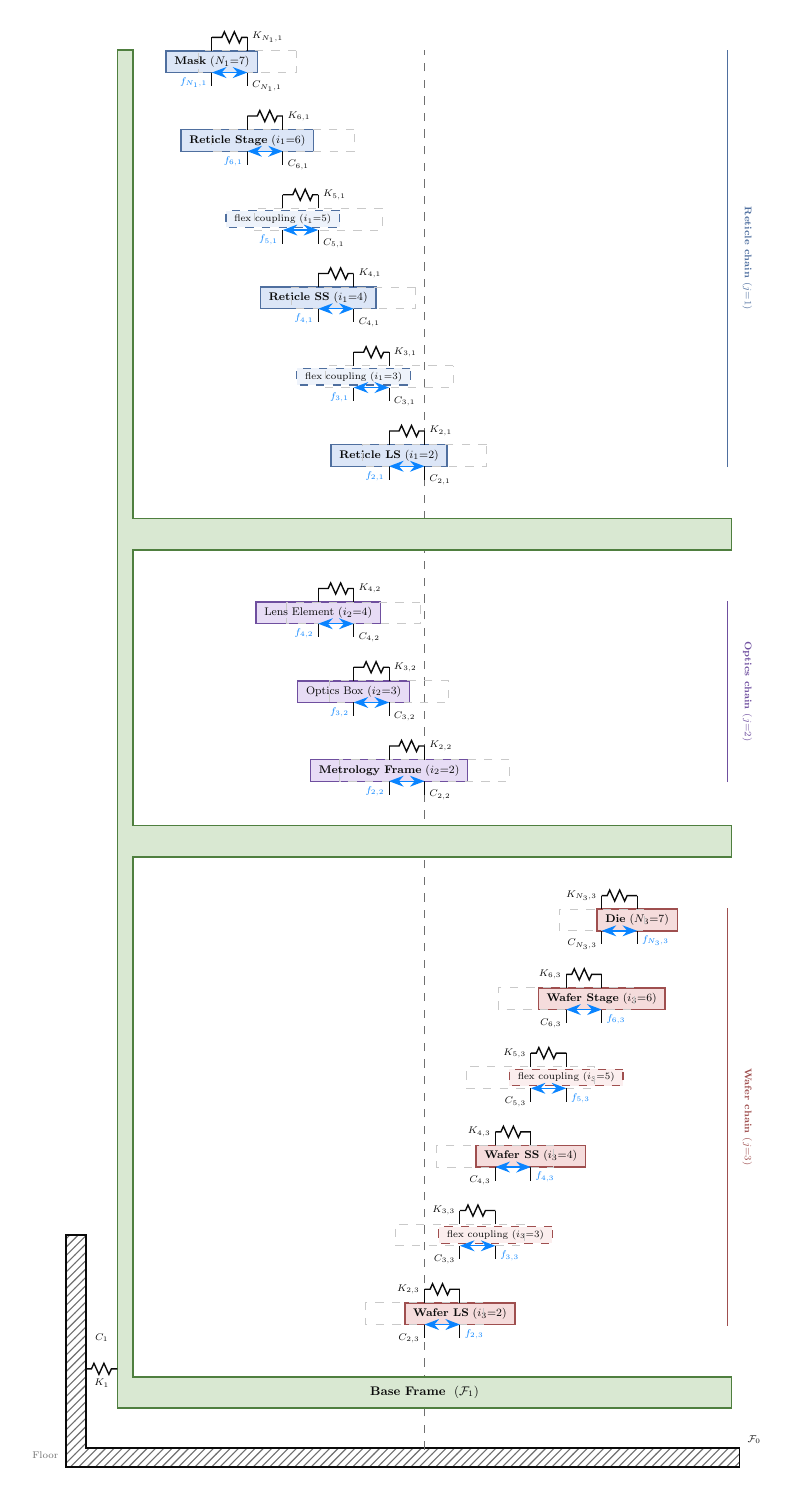
\begin{tikzpicture}[scale=0.5, transform shape,
  every node/.style    ={font=\small},
  rfrm/.style          ={draw=frameEdge, line width=0.6pt, fill=frameFill,
                         minimum height=0.80cm, font=\small\bfseries,
                         inner sep=2pt},
  rblk/.style          ={draw=reticleEdge, line width=0.5pt, fill=reticleFill,
                         minimum height=0.55cm, font=\footnotesize,
                         text=mnnwInk, inner sep=2.5pt},
  rflx/.style          ={draw=reticleEdge, line width=0.4pt, fill=reticleFlex,
                         minimum height=0.42cm, font=\scriptsize,
                         text=mnnwInk, inner sep=2pt, dashed},
  wblk/.style          ={draw=waferEdge, line width=0.5pt, fill=waferFill,
                         minimum height=0.55cm, font=\footnotesize,
                         text=mnnwInk, inner sep=2.5pt},
  wflx/.style          ={draw=waferEdge, line width=0.4pt, fill=waferFlex,
                         minimum height=0.42cm, font=\scriptsize,
                         text=mnnwInk, inner sep=2pt, dashed},
  oblk/.style          ={draw=opticsEdge, line width=0.5pt, fill=opticsFill,
                         minimum height=0.55cm, font=\footnotesize,
                         text=mnnwInk, inner sep=2.5pt},
  oflx/.style          ={draw=opticsEdge, line width=0.4pt, fill=opticsFlex,
                         minimum height=0.42cm, font=\scriptsize,
                         text=mnnwInk, inner sep=2pt, dashed},
  ghost/.style         ={draw=mnnwHair, dashed, line width=0.35pt,
                         fill=none, minimum height=0.55cm},
  hsp/.style           ={line width=0.5pt, mnnwInk, decorate,
                         decoration={zigzag, segment length=3.6pt, amplitude=2pt,
                                     pre length=2pt, post length=2pt}},
  vsp/.style           ={line width=0.5pt, mnnwInk, decorate,
                         decoration={zigzag, segment length=3.6pt, amplitude=2pt,
                                     pre length=2pt, post length=2pt}},
  darr/.style          ={Stealth-Stealth, line width=0.5pt, mnnwSignal},
  lbl/.style           ={font=\scriptsize, text=mnnwInk},
  ftn/.style           ={font=\scriptsize, text=mnnwSignal},
  axis/.style          ={dashed, line width=0.4pt, mnnwMute},
  pillar/.style        ={fill=black!8, draw=mnnwHair, line width=0.3pt},
  hatchfloor/.style    ={pattern=north east lines, pattern color=mnnwMute},
]

% =====================================================================
% Helper macro for one chain body row.
%   #1 y-coord            #2 block-style (rblk/wblk/oblk/rflx/wflx/oflx)
%   #3 previous_x         #4 horizontal offset from Pd (positive = right)
%   #5 block label        #6 K-label   #7 C-label   #8 f-label
% =====================================================================
\newcommand{\chainrow}[8]{%
  % 1. Render the real block first to determine its natural width
  % We use 'inner xsep=6pt' for padding
  \node[#2, inner xsep=6pt] (blk) at (#4,#1) {#5};
  
  % 2. Render the ghost node at the previous x (#3)
  % We use \phantom{#5} so it matches the width/height of the label exactly,
  % but remains completely invisible (empty box)
  \node[ghost, inner xsep=6pt] at (#3,#1) {\phantom{#5}};
  
  % Spring above
  \draw[hsp] (#3, #1+0.62) -- (#4, #1+0.62);
  
  % Anchor lines
  \draw[line width=0.35pt, mnnwInk] (#3, #1+0.275) -- (#3, #1+0.62);
  \draw[line width=0.35pt, mnnwInk] (#4, #1+0.275) -- (#4, #1+0.62);

  % Damper below
  \draw[line width=0.35pt, mnnwInk] (#3, #1-0.275) -- (#3, #1-0.62);
  \draw[line width=0.35pt, mnnwInk] (#4, #1-0.275) -- (#4, #1-0.62);
  
  \hdamperLong{#3}{#4}{#1-0.62}

  % DYNAMIC LABELS (K, C, and f):
  % Logic: If block moves right (#4>#3), place labels on the left (x=#3-0.2, east anchor).
  %        If block moves left (#4<#3), place labels on the right (x=#3+0.2, west anchor).
  \pgfmathsetmacro{\lblSide}{#4 > #3 ? #3 : #3}
  \pgfmathsetmacro{\lblAnch}{#4 > #3 ? "east" : "west"}

  \node[lbl, anchor=\lblAnch] at (\lblSide, #1+0.62) {#6}; % K Label
  \node[lbl, anchor=\lblAnch] at (\lblSide, #1-0.62) {#7}; % C Label
  
  % f label placed at the previous_x axis (#3) but aligned to the same side
  % y-offset of -0.2 matches your deviation arrow's height
  \pgfmathsetmacro{\fSide}{#4 > #3 ? #4 : #4}
  \pgfmathsetmacro{\fAnch}{#4 > #3 ? "west" : "east"}
  \node[ftn, anchor=\fAnch] at (\fSide, #1-0.525) {#8};

  % Deviation arrow (line remains, but label is now at the #3 axis)
  \draw[darr] (#3, #1-0.275) -- (#4, #1-0.275);
}

% =====================================================================
%  GEOMETRY — full stack
% =====================================================================
\def\xLeft{-8.0}\def\xRight{8.0}
\def\xPilL{-7.4}\def\xPilR{7.4}

% Vertical levels (cm). Tight rhythm of 1.6 cm per body row.
% Wafer chain (bodies 2..7 → 6 rows), then F2, then optics (2..4 → 3 rows),
% but per user spec: optics chain attaches around F2 (lens region).
% Layout chosen:
%   F0 floor                  y = 0
%   F1 base frame             y = 1.4
%   Wafer chain  i=2..7       y = 3.2, 4.8, 6.4, 8.0, 9.6, 11.2
%   F2 metrology frame        y = 13.0   (with lens on it)
%   Optics chain  i=2..4      y = 14.4, 15.8, 17.2  (downstream of F2)
%   Reticle chain i=2..7      y = 18.8, 20.4, 22.0, 23.6, 25.2, 26.8
% =====================================================================
\def\yFloor{0}
\def\yBase{1.4}
% Wafer
\def\yWa{3.4}\def\yWb{5.4}\def\yWc{7.4}\def\yWd{9.4}\def\yWe{11.4}\def\yWf{13.4}
% Metrology
% \def\yMet{15.4}
% Optics
\def\yOa{17.2}\def\yOb{19.2}\def\yOc{21.2}
% Reticle
\def\yRa{25.2}\def\yRb{27.2}\def\yRc{29.2}\def\yRd{31.2}\def\yRe{33.2}\def\yRf{35.2}
\def\yTop{35.5}
\def\yShA{15.4}\def\yShB{23.2}

% =====================================================================
%  FLOOR  +  PILLARS  +  Pd
% =====================================================================
\filldraw[hatchfloor, draw=mnnwInk, line width=0.7pt]
  (\xRight, 0) -- (\xLeft-0.6, 0) -- (\xLeft-0.6, \yWb) -- (\xLeft-1.1, \yWb) 
  -- (\xLeft-1.1, -0.5) -- (\xRight, -0.5) -- cycle;
\node[lbl, anchor=west] at (\xRight+0.08,0.20) {$\mathcal{F}_0$};
\node[lbl, anchor=east, text=mnnwMute]
  at (\xLeft-1.1-0.08,-0.18) {Floor};

% \fill[pillar] (\xPilR,0)      rectangle (\xPilR+0.16,\yTop);

\draw[axis] (0,-0.05) -- (0,\yTop);
% \node[font=\small\itshape, anchor=south] at (0,\yTop+0.45) {$P_d$};

% =====================================================================
%  BASE FRAME  F_1
% =====================================================================
\filldraw[draw=frameEdge, line width=0.6pt, fill=frameFill]
  (7.8, \yBase-0.4) -- (-7.8, \yBase-0.4) -- (-7.8, \yTop) -- (-7.4, \yTop)
  -- (-7.4, \yShB+0.4) -- (7.8, \yShB+0.4) -- (7.8, \yShB-0.4) -- (-7.4, \yShB-0.4)
  -- (-7.4, \yShA+0.4) -- (7.8, \yShA+0.4) -- (7.8, \yShA-0.4) -- (-7.4, \yShA-0.4)
  -- (-7.4, \yBase+0.4) -- (7.8, \yBase+0.4) -- cycle;
\node[font=\small\bfseries, text=mnnwInk] at (0, \yBase) {Base Frame $\;(\mathcal{F}_1)$};

% K_1 / C_1  horizontal floor → base frame
\def\lblX{\xLeft-1.2} 

% 1. The Spring (K1)
\hdamperLong{\xLeft-0.6}{-7.8}{2.5}
\node[lbl, above=2pt] at ({(\xLeft-0.6-7.8)/2}, 2.5) {$C_1$};

% 2. The Spring (K1) - Placed on bottom
\draw[hsp] (\xLeft-0.6, 2.0) -- (-7.8, 2.0)
  node[midway, below=4pt, lbl] {$K_1$};

% =====================================================================
%  WAFER CHAIN  (j=3) — light red, blocks shifted RIGHT of Pd
%  i = 2 LS, 3 LS-flex, 4 MS, 5 MS-flex, 6 SS, 7 wafer (N3)
% =====================================================================
\chainrow{\yWa}{wblk}{0}{ 0.9}{\textbf{Wafer LS} $(i_3{=}2)$}{$K_{2,3}$}{$C_{2,3}$}{$f_{2,3}$}
\chainrow{\yWb}{wflx}{0.9}{ 1.8}{flex coupling $(i_3{=}3)$}{$K_{3,3}$}{$C_{3,3}$}{$f_{3,3}$}
\chainrow{\yWc}{wblk}{1.8}{ 2.7}{\textbf{Wafer SS} $(i_3{=}4)$}{$K_{4,3}$}{$C_{4,3}$}{$f_{4,3}$}
\chainrow{\yWd}{wflx}{2.7}{ 3.6}{flex coupling $(i_3{=}5)$}{$K_{5,3}$}{$C_{5,3}$}{$f_{5,3}$}
\chainrow{\yWe}{wblk}{3.6}{ 4.5}{\textbf{Wafer Stage} $(i_3{=}6)$}{$K_{6,3}$}{$C_{6,3}$}{$f_{6,3}$}
\chainrow{\yWf}{wblk}{4.5}{ 5.4}{\textbf{Die} $(N_3{=}7)$}{$K_{N_3,3}$}{$C_{N_3,3}$}{$f_{N_3,3}$}

% =====================================================================
%  METROLOGY FRAME  F_2  +  Lens body
% =====================================================================
% \node[rfrm, minimum width=13cm, minimum height=1.0cm] (MF) at (0,\yMet)
%   {Metrology Frame $\;(\mathcal{F}_2)$};
% \node[draw=mnnwInk, line width=0.4pt, fill=lensFill,
%       minimum width=2.4cm, minimum height=0.40cm,
%       font=\scriptsize, anchor=south] at (0,\yMet+0.55) {Lens cell};
% \draw[line width=0.3pt, mnnwInk] (-0.40,\yMet+0.55) -- (-0.75,\yMet+1.05);
% \draw[line width=0.3pt, mnnwInk] ( 0.40,\yMet+0.55) -- ( 0.75,\yMet+1.05);
% \draw[line width=0.3pt, mnnwInk] (-0.40,\yMet-0.10) -- (-0.75,\yMet-0.65);
% \draw[line width=0.3pt, mnnwInk] ( 0.40,\yMet-0.10) -- ( 0.75,\yMet-0.65);

% K_2 / C_2  horizontal pillar → metrology (left side)
% \draw[hsp] (-7.4, \yMet+0.25) -- (-6.5, \yMet+0.25)
%   node[midway, above=2pt, lbl] {$K_{2,2}$};
% \hdamperLong{-7.4}{-6.5}{\yMet-0.25}
% \node[lbl, below] at (-6.95, \yMet-0.38) {$C_{2,2}$};

% =====================================================================
%  OPTICS CHAIN  (j=2)  — light purple, blocks shifted LEFT of Pd
%  Modeled as a 4-body chain whose first body (i=2) attaches to F2.
%  i = 2 lens-frame coarse, i = 3 flex, i = 4 lens cell (N2).
%  Drawn UPWARD from F2 toward the optical axis region.
% =====================================================================
\chainrow{\yOa}{oblk}{0}{-0.9}{\textbf{Metrology Frame} $(i_2{=}2)$}{$K_{2,2}$}{$C_{2,2}$}{$f_{2,2}$}
\chainrow{\yOb}{oblk}{-0.9}{-1.8}{Optics Box $(i_2{=}3)$}{$K_{3,2}$}{$C_{3,2}$}{$f_{3,2}$}
\chainrow{\yOc}{oblk}{-1.8}{-2.7}{Lens Element $(i_2{=}4)$}{$K_{4,2}$}{$C_{4,2}$}{$f_{4,2}$}

% =====================================================================
%  RETICLE CHAIN  (j=1) — light blue, blocks shifted LEFT of Pd
%  i = 2 LS, 3 LS-flex, 4 MS, 5 MS-flex, 6 SS, 7 mask (N1)
% =====================================================================
\chainrow{\yRa}{rblk}{0}{-0.9}{\textbf{Reticle LS} $(i_1{=}2)$}{$K_{2,1}$}{$C_{2,1}$}{$f_{2,1}$}
\chainrow{\yRb}{rflx}{-0.9}{-1.8}{flex coupling $(i_1{=}3)$}{$K_{3,1}$}{$C_{3,1}$}{$f_{3,1}$}
\chainrow{\yRc}{rblk}{-1.8}{-2.7}{\textbf{Reticle SS} $(i_1{=}4)$}{$K_{4,1}$}{$C_{4,1}$}{$f_{4,1}$}
\chainrow{\yRd}{rflx}{-2.7}{-3.6}{flex coupling $(i_1{=}5)$}{$K_{5,1}$}{$C_{5,1}$}{$f_{5,1}$}
\chainrow{\yRe}{rblk}{-3.6}{-4.5}{\textbf{Reticle Stage} $(i_1{=}6)$}{$K_{6,1}$}{$C_{6,1}$}{$f_{6,1}$}
\chainrow{\yRf}{rblk}{-4.5}{-5.4}{\textbf{Mask} $(N_1{=}7)$}{$K_{N_1,1}$}{$C_{N_1,1}$}{$f_{N_1,1}$}

% =====================================================================
%  CHAIN BRACES  (right edge — quick orienteering)
% =====================================================================
\draw[line width=0.4pt, waferEdge]   (\xPilR+0.30,\yWa-0.30) -- (\xPilR+0.30,\yWf+0.30);
\node[font=\scriptsize\bfseries, text=waferEdge, rotate=-90, anchor=south]
  at (\xPilR+0.55,{(\yWa+\yWf)/2}) {Wafer chain $(j{=}3)$};
\draw[line width=0.4pt, opticsEdge]  (\xPilR+0.30,\yOa-0.30) -- (\xPilR+0.30,\yOc+0.30);
\node[font=\scriptsize\bfseries, text=opticsEdge, rotate=-90, anchor=south]
  at (\xPilR+0.55,{(\yOa+\yOc)/2}) {Optics chain $(j{=}2)$};
\draw[line width=0.4pt, reticleEdge] (\xPilR+0.30,\yRa-0.30) -- (\xPilR+0.30,\yRf+0.30);
\node[font=\scriptsize\bfseries, text=reticleEdge, rotate=-90, anchor=south]
  at (\xPilR+0.55,{(\yRa+\yRf)/2}) {Reticle chain $(j{=}1)$};

\end{tikzpicture}
\caption{Lumped mass-spring-damper system of the three chains vertically stacked on the common base frame}
\label{fig:litho_model_full}
\end{figure}

The \emph{wafer chain} ($j=3$, $N_3=7$,
red) below, the \emph{optics chain} ($j=2$, $N_2=4$, purple) attached to
the metrology frame $\mathcal{F}_2$, and the \emph{reticle chain} ($j=1$,
$N_1=7$, blue) above. Solid blocks denote actuated stages
($i\in\{2,4,6\}$ — LS, MS, SS) and the end-effectors ($i=N_j$); dashed
blocks denote passive flex couplings ($i\in\{3,5,7\}$). The dashed
vertical centerline is the intended trajectory from which horizontal blue
double-headed arrows label the in-plane deviation $f_{i,j}$ of each body
from it. Horizontal Kelvin–Voigt elements $(K_{i,j},C_{i,j})$ couple
each stage laterally to the fixed structural reference; Kelvin–Voigt
elements $(K_1,C_1)$ and $(K_2,C_2)$ provide passive vibration isolation between
$\mathcal{F}_0\!\rightarrow\!\mathcal{F}_1$ and
$\mathcal{F}_1\!\rightarrow\!\mathcal{F}_2$.

\section{Model}

In \cite{Al-Rawashdeh2022_Caracterization}, the authors propose modeling the lithography scanner as a combination of three open-loop serial chains: the reticle chain ($j=1$), the optics chain ($j=2$), and the wafer chain ($j=3$), the latter being of primary interest for the step-and-scan motion problem studied here.

The full 6-DOF model of \cite{Al-Rawashdeh2022_Caracterization} is here restricted to in-plane (planar) motions. The generalized coordinate used to describe the configuration of the $i$th stage within the $j$th chain is
\begin{equation}
    q_{i_j} = \begin{bmatrix} f_{i_j} \\ \theta_{z_{i_j}} \end{bmatrix} \in \mathbb{R}^{3\times1},
\end{equation}
where $f_{i_j} = [f_{x,i_j},\, f_{y,i_j}]^T \in \mathbb{R}^{2}$ collects the in-plane translational displacements of stage $i$ \emph{relative to its parent body} in chain $j$, and $\theta_{z_{i_j}} \in \mathbb{R}$ is the corresponding rotation about the out-of-plane $z$-axis. The joints between bodies within a chain are modeled as a low-mass Kelvin--Voigt element — a parallel spring-damper system \cite{Al-Rawashdeh2022_Caracterization}. Two distinct joint types arise: \emph{actuated} stages ($i \in \{2,4,6\}$), which are driven by servo motors and carry a near-infinite effective stiffness that keeps $f_{i_j}$ locked to the commanded trajectory; and \emph{flex} stages ($i \in \{3,5,7\}$), which are passive compliant connections whose stiffness $K_{i_j}$ and damping $C_{i_j}$ are physical material properties of the mechanical coupling. The associated generalized mass-inertia matrix for each body is
\begin{equation}
    M_{i_j} = \begin{bmatrix} m_{i_j}\,\mathbf{I}_2 & 0 \\ 0 & I_{z_{i_j}} \end{bmatrix} \in \mathbb{R}^{3\times3},
\end{equation}
and the generalized stiffness and damping matrices $K_{i_j},\, C_{i_j} \in \mathbb{R}^{3\times3}$ are block-diagonal, with a $2\times2$ translational block and a scalar rotational entry.

In order to recover the absolute (inertial-frame) position $f^{0}_{i_j}$ of body $i$ from its relative joint coordinates, one accumulates the relative displacements along the chain from the floor frame $\mathcal{F}_{0}$. For bodies with $i \geq 2$ on any chain $j \in \{1,2,3\}$:
\begin{equation} \label{eq:frameref}
    f^{0}_{i_j} = f^{0}_{(i-1)_j} + f_{i_j}
\end{equation}

Since the rotation about the $z$-axis is a scalar, the angular position recurrence is simply additive:
\begin{equation} \label{eq:angleref}
    \theta^{0}_{z_{i_j}} = \theta^{0}_{z_{(i-1)_j}} + \theta_{z_{i_j}}
\end{equation}

The translational velocity expression appears as:
\begin{equation}
    \dot{f}^{0}_{i_j} = \dot{f}^{0}_{(i-1)_j} + \dot{f}_{i_j} + \omega_{(i-1)_j}
    \times
    f_{i_j}
\end{equation}

Where $\omega_{(i-1)_j}$ is the angular velocity \supercite{Ginsberg1984_AdvancedDynamics} of $\mathcal{F}_{(i-1)_j}$ with respect to the floor, $\mathcal{F}_{0}$.

Taking the second derivative gives:
\begin{align}
    \begin{split}
        \ddot{f}^{0}_{i_j} &= \ddot{f}^{0}_{(i-1)_j} + \ddot{f}_{i_j}
        + \omega_{(i-1)_j} \times \dot{f}_{i_j}
        + \dot{\omega_{(i-1)_j}} \times f_{i_j}
        + \omega_{(i-1)_j} \times \left[
            \dot{f}_{i_j} + \omega_{(i-1)_j} \times f_{i_j}
        \right] \\
        &= \ddot{f}^{0}_{(i-1)_j} + \ddot{f}_{i_j}
        + \omega_{(i-1)_j} \times \dot{f}_{i_j}
        + \dot{\omega_{(i-1)_j}} \times f_{i_j}
        + \omega_{(i-1)_j} \times \dot{f}_{i_j}
        + \omega_{(i-1)_j} \times \left[
            \omega_{(i-1)_j} \times f_{i_j}
        \right] \\
        &= \ddot{f}^{0}_{(i-1)_j} + \ddot{f}_{i_j}
        + 2 \left[ \omega_{(i-1)_j} \times \dot{f}_{i_j} \right]
        + \dot{\omega_{(i-1)_j}} \times f_{i_j}
        + \omega_{(i-1)_j} \times \left[
            \omega_{(i-1)_j} \times f_{i_j}
        \right]
    \end{split}
\end{align}

Since we are concerned with planar movements in this work, we restrict the angular velocity of each body purely about the $z$-axis as $\omega = \dot{\theta}_z\,\hat{z}$, so that:
\begin{equation}
    \omega_{(i-1)_j} = \dot{\theta}^{0}_{z_{(i-1)_j}}\,\hat{z} \notag
\end{equation}

We substitute the cross-products as matrix-vector products using the skew-symmetric matrix. In \cite{Al-Rawashdeh2022_Caracterization}, it appears as:
\begin{equation}
    [\omega]
    =
    \begin{bmatrix}
        0 & -\omega_z & \omega_y \\
        \omega_z & 0 & -\omega_x \\
        -\omega_y & \omega_x & 0
    \end{bmatrix}
    \notag
\end{equation}
Clearly, here we can set $\omega_x = 0$ and $\omega_y = 0$, thus $\omega = [0,\, 0,\, \dot{\theta}_z]^T$ the matrix becomes:
\begin{equation}
    [\omega]
    =
    \begin{bmatrix}
        0 & -\omega_z & 0 \\
        \omega_z & 0 & 0 \\
        0 & 0 & 0
    \end{bmatrix}
    \notag
\end{equation}

Considering our 2D displacement vector, we only take the upper-left $2\times2$ 
sub-matrix, and factoring out the scalar $\dot{\theta}^{0}_{z_{(i-1)_j}}$:
\begin{equation} \label{eq:skew}
    [\omega_{(i-1)_j}] = \dot{\theta}^{0}_{z_{(i-1)_j}}
    \begin{bmatrix} 0 & -1 \\ 1 & 0 \end{bmatrix}
\end{equation}
such that $\omega_{(i-1)_j} \times f_{i_j} = [\omega_{(i-1)_j}]\,f_{i_j}$. 
Applying this matrix twice gives the centripetal term:
\begin{equation}
    [\omega_{(i-1)_j}]^2 = -\left(\dot{\theta}^{0}_{z_{(i-1)_j}}\right)^2 \mathbf{I}_2
\end{equation}
so that $\omega_{(i-1)_j} \times [\omega_{(i-1)_j} \times f_{i_j}] =
[\omega_{(i-1)_j}]^2\,f_{i_j}$. Substituting and expanding
\eqref{eq:frameref} recursively from the floor frame, the translational kinematics become:
\begin{align}
    f^{0}_{i_j}
        &= f^{0}_{1} + \sum^{i}_{k=2} f_{k_j}
        \label{eq:pos_expanded} \\
    \dot{f}^{0}_{i_j}
        &= \dot{f}^{0}_{1} + \sum^{i}_{k=2} \dot{f}_{k_j}
         + \sum^{i}_{k=2} [\omega_{(k-1)_j}]\, f_{k_j}
        \label{eq:vel_expanded} \\
    \ddot{f}^{0}_{i_j}
        &= \ddot{f}^{0}_{1} + \sum^{i}_{k=2} \ddot{f}_{k_j}
         + \sum^{i}_{k=2} \left[
             2\,[\omega_{(k-1)_j}]\,\dot{f}_{k_j}
             + [\dot{\omega}_{(k-1)_j}]\,f_{k_j}
             + [\omega_{(k-1)_j}]^2\,f_{k_j}
         \right]
        \label{eq:acc_expanded}
\end{align}

Since the rotation $\theta_{z_{i_j}}$ is a scalar, no Coriolis or centripetal cross-terms arise in the angular kinematics. Expanding \eqref{eq:angleref} recursively from the floor frame gives the rotational analogues:
\begin{align}
    \theta^{0}_{z_{i_j}}
        &= \theta^{0}_{z_1} + \sum^{i}_{k=2} \theta_{z_{k_j}}
        \label{eq:angle_expanded} \\
    \dot{\theta}^{0}_{z_{i_j}}
        &= \dot{\theta}^{0}_{z_1} + \sum^{i}_{k=2} \dot{\theta}_{z_{k_j}}
        \label{eq:angvel_expanded} \\
    \ddot{\theta}^{0}_{z_{i_j}}
        &= \ddot{\theta}^{0}_{z_1} + \sum^{i}_{k=2} \ddot{\theta}_{z_{k_j}}
        \label{eq:angacc_expanded}
\end{align}

Thus the equation of the angular motion of the $i$th body in the $j$th chain w.r.t $\mathcal{F}_{0}$ is:
\begin{equation}
    {}^{0}\!I_j \, \dot{\omega}_j + \left( [\omega_j] \right) {}^{0}\!I_j \, \omega_j  = m_j^0
\end{equation}

Under the planar restriction $\omega_x = \omega_y = 0$ the gyroscopic term vanishes like:
\begin{equation}
    \left([\omega_{i_j}]\,{}^0\!I_{i_j}\right)\omega_{i_j}
    =
    \begin{bmatrix}
        0 & -\dot{\theta}_z & 0 \\
        \dot{\theta}_z & 0 & 0 \\
        0 & 0 & 0
    \end{bmatrix}
    \begin{bmatrix}
        I_{xx} & 0 & 0 \\
        0 & I_{yy} & 0 \\
        0 & 0 & I_{zz}
    \end{bmatrix}
    \begin{bmatrix}
        0 \\
        0 \\
        \dot{\theta}_z
    \end{bmatrix}
    = 0
    \notag
\end{equation}

Leaving only:
\begin{equation}
    I_{z_{i_j}}\ddot{\theta}^{0}_{z_{i_j}} = m^0_{z_{i_j}}
\end{equation}

where $I_{z_{i_j}}$ is the aggregated moment of inertia of all bodies from $i$ to the end-effector $N_j$, referred to the $z$-axis of body $i$ via Steiner's theorem, and $m^0_{z_{i_j}} \in \mathbb{R}$ is the net applied moment acting on body $i$ in chain $j$ about the $z$-axis.

\paragraph{Steiner's theorem and inertia aggregation.}
The parallel axis (Steiner's) theorem states that the moment of inertia of a rigid body about any axis parallel to one through its center of mass (CoG) satisfies
\begin{equation} \label{eq:steiner}
    I_z = \tilde{I}_z + m\,\|f\|^2,
\end{equation}
where $\tilde{I}_z$ is the body's own moment of inertia about the $z$-axis through its CoG, $m$ is its mass, and $\|f\|^2 = f_x^2 + f_y^2$ is the squared in-plane distance between the two parallel axes. In a serial chain, the inertia of every downstream body must be shifted to the frame of the current body using \eqref{eq:steiner}. Following \cite{Al-Rawashdeh2022_Caracterization} (Algorithm~1 therein), the aggregated inertia for the $j$th chain is computed recursively from the end-effector inward. In the planar restriction, the full $3\times3$ inertia matrix of the original algorithm reduces to a scalar $z$-axis inertia:

\begin{algorithm}[H]
\caption{Planar inertia aggregation for the $j$th chain — planar reduction of Algorithm~1 in \cite{Al-Rawashdeh2022_Caracterization}}
\begin{algorithmic}[1]
\Require{CoG inertias $\tilde{I}_{z_{i_j}}$, masses $m_{i_j}$, relative positions $f_{k_j}$ for $i = 2,\ldots,N_j$}
\Ensure{Aggregated inertias $^0I_{z_{i_j}}$ for $i = 2,\ldots,N_j$}
\State \textbf{Initialize:} $^0I_{z_{N_j}} \leftarrow \tilde{I}_{z_{N_j}}$
\If{$2 \leq i < N_j$}
    \For{$k = N_j,\;\ldots,\;i+1$}
        \State $\tilde{m}_{(k-1)_j} \leftarrow \displaystyle\sum_{b=k}^{N_j} m_{b_j}$
        \Comment{accumulated downstream mass}
        \State $^0I_{z_{(k-1)_j}} \leftarrow {}^0I_{z_{k_j}} + \tilde{I}_{z_{(k-1)_j}} + \tilde{m}_{(k-1)_j}\bigl(f_{x,k_j}^2 + f_{y,k_j}^2\bigr)$
        \Comment{Steiner shift from frame $k$ to frame $k\!-\!1$}
    \EndFor
\EndIf
\end{algorithmic}
\end{algorithm}

Here $\tilde{m}_{(k-1)_j} = \sum_{b=k}^{N_j} m_{b_j}$ is the total mass of all downstream bodies (from $k$ to the end-effector), $\tilde{I}_{z_{(k-1)_j}}$ is the local inertia of body $k-1$ about its own CoG, and $\tilde{m}_{(k-1)_j}(f_{x,k_j}^2 + f_{y,k_j}^2)$ is the Steiner correction that shifts the accumulated inertia from body $k$'s CoG to body $(k-1)$'s CoG. By the time the algorithm terminates, $^0I_{z_{2_j}}$ contains the inertia of the entire chain $j$ referred to the CoG of its first body.

The aggregated inertia of the base frame (body~1) applies the same shift one more time, from body~2's CoG to the base frame:
\begin{equation} \label{eq:Iz0}
    {}^0I_{z_1} = \tilde{I}_{z_1}
    + \sum_{j=1}^{3}\!\Bigl({}^0I_{z_{2_j}}
      + \tilde{m}_{1_j}\bigl(f_{x,2_j}^2 + f_{y,2_j}^2\bigr)\Bigr),
\end{equation}
where $\tilde{m}_{1_j} = \sum_{b=2}^{N_j} m_{b_j}$ is the total mass of chain $j$. This is the quantity denoted $I_{z_0}$ in \eqref{eq:baseframerot}.

Expanding $\ddot{\theta}^0_{z_{i_j}}$ using \eqref{eq:angacc_expanded}:
\begin{equation} \label{eq:torqueeq_expanded}
    I_{z_{i_j}}\ddot{\theta}^{0}_{z_1} 
    + I_{z_{i_j}}\sum^{i}_{k=2}\ddot{\theta}_{z_{k_j}}
    = m^0_{z_{i_j}}
\end{equation}

\subsection{For the base frame}

To write the equations that govern the base frame, we start from Newton's equation $F = ma$. For every body ($i \geq 2$) within chain $j$, it connects to body $i-1$ through a spring above and body $i+1$ through the spring below:
\begin{align} \label{eq:forceeq}
    \begin{split}
        m_{i_j}\ddot{f}^{0}_{1}
        + m_{i_j}\sum^{i}_{k=2}\ddot{f}_{k_j}
        + m_{i_j}\sum^{i}_{k=2}
        &\left[
            2\,[\omega_{(k-1)_j}]\,\dot{f}_{k_j}
            + [\dot{\omega}_{(k-1)_j}]\,f_{k_j}
            + [\omega_{(k-1)_j}]^2\,f_{k_j}
        \right] \\
        - K_i\left( f^0_{{(i-1)}_j} - f^0_{{i}_j}\right)
        - C_i\left( \dot{f}^0_{{(i-1)}_j} - \dot{f}^0_{{i}_j}\right)
        &+ K_{i+1}\left( f^0_{{i}_j} - f^0_{{(i+1)}_j}\right)
        + C_{i+1}\left( \dot{f}^0_{{i}_j} - \dot{f}^0_{{(i+1)}_j}\right)
        = u^0_{i_j}
    \end{split}
\end{align}

Summing \eqref{eq:forceeq} over all bodies in a chain (taking the optics chain $j=2$, bodies $i=2,3,4$ as a representative example), the internal spring forces cancel by Newton's third law:
\begin{align}
    &- K_2(f^0_1 - f^0_2) - C_2(\dot{f}^0_1 - \dot{f}^0_2) \notag \\
    &\quad \cancelto{0}{
        + K_3(f^0_2 - f^0_3) + C_3(\dot{f}^0_2 - \dot{f}^0_3)
        - K_3(f^0_2 - f^0_3) - C_3(\dot{f}^0_2 - \dot{f}^0_3)
    } \notag \\
    &\quad \cancelto{0}{
        + K_4(f^0_3 - f^0_4) + C_4(\dot{f}^0_3 - \dot{f}^0_4)
        - K_4(f^0_3 - f^0_4) - C_4(\dot{f}^0_3 - \dot{f}^0_4)
    } \notag
\end{align}

Only the boundary term $- K_2(f^0_1 - f^0_2) - C_2(\dot{f}^0_1 - \dot{f}^0_2)$ survives, which corresponds to the connection between body $i = 2$ and the base frame. This extends to any $N_j$-body chain. Recalling \eqref{eq:frameref}, $f^{0}_{1} - f^{0}_{2_j} = -f_{2_j}$, and following \cite{Al-Rawashdeh2022_Caracterization} with ${}^0K_{i_j}={}^0R_{i_j} K_{i_j} {}^0R^T_{i_j}$ and ${}^0C_{i_j}={}^0R_{i_j} C_{i_j} {}^0R^T_{i_j}$, the total translational equation of the base frame (absorbing the balance masses and collecting all chain contributions) is:
\begin{align} \label{eq:baseframeeq}
    \begin{split}
        m_0\,\ddot{f}^{0}_{1}
        + {}^0\bar{C}_1\,\dot{f}_1
        + {}^0\bar{K}_1\,f_1
        - \sum_{j=1}^{3}\left\{
            {}^0\bar{C}_{2_j}\,\dot{f}_{2_j} + {}^0\bar{K}_{2_j}\,f_{2_j}
        \right\}
        &= u^0_{1}
    \end{split}
\end{align}
where $m_0 = m_{1} + \sum_{j=1}^{3}\!\left(m^j_{B} + \sum_{i=2}^{N_j} m_{i_j}\right)$ is the total system mass, and the stiffness and damping matrices denote the $2\times2$ translational block.

By the exact same cancellation argument applied to the moment balance about the $z$-axis — the moment exerted by the spring connecting body $i$ to body $i-1$ is $-K_{i_j}\,\theta_{z_{i_j}}$, so internal moments cancel identically — the rotational equation of the base frame is:
\begin{align} \label{eq:baseframerot}
    \begin{split}
        I_{z_0}\,\ddot{\theta}^{0}_{z_1}
        + {}^0\bar{C}_1\,\dot{\theta}_{z_1}
        + {}^0\bar{K}_1\,\theta_{z_1}
        - \sum_{j=1}^{3}\left\{
            {}^0\bar{C}_{2_j}\,\dot{\theta}_{z_{2_j}}
            + {}^0\bar{K}_{2_j}\,\theta_{z_{2_j}}
        \right\}
        &= \tau^0_{1}
    \end{split}
\end{align}
where $I_{z_0} = I_{z_1} + \sum_{j=1}^{3}\!\left(I^j_{z_B} + \sum_{i=2}^{N_j} I_{z_{i_j}}\right)$ is the total moment of inertia of the system about the $z$-axis, ${}^0\bar{C}_{i_j}$ and ${}^0\bar{K}_{i_j}$ are the scalar rotational damping and stiffness of the joint connecting body $i$ to its predecessor in chain $j$, and $\tau^0_1$ is the net applied torque on the base frame.

\subsection{For each chain}

Recalling \eqref{eq:forceeq} and \eqref{eq:torqueeq_expanded}, for the first body in the chain ($i=2$), which connects to the base frame above and to body $i=3$ below, the translational equation is:
\begin{equation}
        \bar{m}_{2_j}
        \ddot{f}^{0}_{2_j}
        + {}^0\bar{C}_{2_j}\,\dot{f}_{2_j}
        + {}^0\bar{K}_{2_j}\,f_{2_j}
        - \left\{
            {}^0\bar{C}_{3_j}\,\dot{f}_{3_j} + {}^0\bar{K}_{3_j}\,f_{3_j}
        \right\}
        = u^0_{2_j}
\end{equation}
and the rotational equation is:
\begin{equation}
        I_{z_{2_j}}\ddot{\theta}^{0}_{z_{2_j}}
        + {}^0\bar{C}_{2_j}\,\dot{\theta}_{z_{2_j}}
        + {}^0\bar{K}_{2_j}\,\theta_{z_{2_j}}
        - {}^0\bar{C}_{3_j}\,\dot{\theta}_{z_{3_j}}
        - {}^0\bar{K}_{3_j}\,\theta_{z_{3_j}}
        = \tau^0_{2_j}
\end{equation}

For bodies $3\leq i< N_j$, the same structure holds with bodies $2, \dots, i-1$ in between. The translational equation is:
\begin{equation}
        \bar{m}_{i_j}
        \ddot{f}^{0}_{i_j}
        + {}^0\bar{C}_{i_j}\,\dot{f}_{i_j}
        + {}^0\bar{K}_{i_j}\,f_{i_j}
        -
        \left\{
            {}^0\bar{C}_{(i+1)_j}\,\dot{f}_{(i+1)_j} + {}^0\bar{K}_{(i+1)_j}\,f_{(i+1)_j}
        \right\}
        = u^0_{i_j}
\end{equation}
and the rotational equation is:
\begin{equation}
        I_{z_{i_j}}\ddot{\theta}^{0}_{z_{i_j}}
        + {}^0\bar{C}_{i_j}\,\dot{\theta}_{z_{i_j}}
        + {}^0\bar{K}_{i_j}\,\theta_{z_{i_j}}
        - {}^0\bar{C}_{(i+1)_j}\,\dot{\theta}_{z_{(i+1)_j}}
        - {}^0\bar{K}_{(i+1)_j}\,\theta_{z_{(i+1)_j}}
        = \tau^0_{i_j}
\end{equation}

Finally, for body $i = N_j$ (the end effector), there is no subsequent body in the chain. The translational and rotational equations are:
\begin{equation}
        \bar{m}_{{N_j}_j}
        \ddot{f}^{0}_{{N_j}_j}
        + {}^0\bar{C}_{{N_j}_j}\,\dot{f}_{{N_j}_j}
        + {}^0\bar{K}_{{N_j}_j}\,f_{{N_j}_j}
        = 0
\end{equation}
\begin{equation}
        I_{z_{{N_j}_j}}\ddot{\theta}^{0}_{z_{{N_j}_j}}
        + {}^0\bar{C}_{{N_j}_j}\,\dot{\theta}_{z_{{N_j}_j}}
        + {}^0\bar{K}_{{N_j}_j}\,\theta_{z_{{N_j}_j}}
        = 0
\end{equation}

\subsection{State-space formulation}

Because each body possesses three planar degrees of freedom ($f_x$, $f_y$, $\theta_z$) along with their corresponding time derivatives, it contributes exactly six states to the system. Following the framework outlined in Appendix~B of \cite{Al-Rawashdeh2022_Caracterization}, the complete machine model comprises 6 bodies in the reticle chain ($N_1 = 7$), 3 bodies in the optics chain ($N_2 = 4$), and 6 bodies in the wafer chain ($N_3 = 7$). Including the common base frame (body 1), the system features a total of $1 + (N_1-1) + (N_2-1) + (N_3-1) = 16$ bodies. Consequently, the global state vector $x$ encompasses $6 \times 16 = 96$ states:

\begin{equation}
    x =
    \begin{bmatrix}
        \underbrace{x_1, \ldots, x_6}_{\text{base frame}} \;,\;
        \underbrace{x_7, \ldots, x_{6N_1}}_{\text{chain 1: bodies } 2 \to N_1} \;,\;
        \underbrace{\ldots}_{\text{chain 2}} \;,\;
        \underbrace{\ldots}_{\text{chain 3}}
    \end{bmatrix}^T
\end{equation}

The explicit mapping for each state is detailed in the table below. Here, $p$ denotes the global sequential index of the $i$-th body in the $j$-th chain within the concatenated list of all bodies (starting with the base frame, followed sequentially by chains 1, 2, and 3). It is crucial to note that every positional entry within the state vector represents a \emph{relative} joint displacement; the corresponding absolute inertial position $f^0_{i_j}$ can be reconstructed using the recursive summations from \eqref{eq:pos_expanded} to \eqref{eq:angle_expanded}.

\begin{center}
\begin{tabular}{cll}
\toprule
State-space Variable & Expression & Meaning \\
\midrule
$x_1$       & $f_{x_1}$                  & base frame $x$-position \\
$x_2$       & $f_{y_1}$                  & base frame $y$-position \\
$x_3$       & $\theta_{z_1}$             & base frame rotation \\
$x_4$       & $\dot{f}_{x_1}$            & base frame $x$-velocity \\
$x_5$       & $\dot{f}_{y_1}$            & base frame $y$-velocity \\
$x_6$       & $\dot{\theta}_{z_1}$       & base frame angular velocity \\
$x_7$       & $f_{x_{2_1}}$              & chain 1, body 2, $x$-position \\
$x_8$       & $f_{y_{2_1}}$              & chain 1, body 2, $y$-position \\
$x_9$       & $\theta_{z_{2_1}}$         & chain 1, body 2, rotation \\
$x_{10}$    & $\dot{f}_{x_{2_1}}$        & chain 1, body 2, $x$-velocity \\
$x_{11}$    & $\dot{f}_{y_{2_1}}$        & chain 1, body 2, $y$-velocity \\
$x_{12}$    & $\dot{\theta}_{z_{2_1}}$   & chain 1, body 2, angular velocity \\
$\vdots$    & $\vdots$                   & $\vdots$ \\
$x_{6p-5}$  & $f_{x_{i_j}}$              & chain $j$, body $i$, $x$-position \\
$x_{6p-4}$  & $f_{y_{i_j}}$              & chain $j$, body $i$, $y$-position \\
$x_{6p-3}$  & $\theta_{z_{i_j}}$         & chain $j$, body $i$, rotation \\
$x_{6p-2}$  & $\dot{f}_{x_{i_j}}$        & chain $j$, body $i$, $x$-velocity \\
$x_{6p-1}$  & $\dot{f}_{y_{i_j}}$        & chain $j$, body $i$, $y$-velocity \\
$x_{6p}$    & $\dot{\theta}_{z_{i_j}}$   & chain $j$, body $i$, angular velocity \\
$\vdots$    & $\vdots$                   & $\vdots$ \\
\bottomrule
\end{tabular}
\end{center}

Solving \eqref{eq:baseframeeq} and \eqref{eq:baseframerot} for the base-frame accelerations yields:
\begin{align}
    \ddot{f}^{0}_{1}
    &= -\frac{{}^0\bar{C}_1}{m_0}\,\dot{f}_1
       -\frac{{}^0\bar{K}_1}{m_0}\,f_1
       +\frac{1}{m_0}\sum_{j=1}^{3}\left\{
           {}^0\bar{C}_{2_j}\,\dot{f}_{2_j} + {}^0\bar{K}_{2_j}\,f_{2_j}
       \right\}
       +\frac{u^0_{1}}{m_0} \label{eq:f1ddot} \\[4pt]
    \ddot{\theta}^{0}_{z_1}
    &= -\frac{{}^0\bar{C}_1}{I_{z_0}}\,\dot{\theta}_{z_1}
       -\frac{{}^0\bar{K}_1}{I_{z_0}}\,\theta_{z_1}
       +\frac{1}{I_{z_0}}\sum_{j=1}^{3}\left\{
           {}^0\bar{C}_{2_j}\,\dot{\theta}_{z_{2_j}} + {}^0\bar{K}_{2_j}\,\theta_{z_{2_j}}
       \right\}
       +\frac{\tau^0_{1}}{I_{z_0}} \label{eq:th1ddot}
\end{align}

Expressed in the standard matrix form $\dot{x} = Ax + Bu$, the first six rows governing the base-frame dynamics are:
\setcounter{MaxMatrixCols}{20}
\begin{equation}
\begin{bmatrix}\dot{x}_1\\\dot{x}_2\\\dot{x}_3\\\dot{x}_4\\\dot{x}_5\\\dot{x}_6\end{bmatrix}
=
\begin{bmatrix}
    0 & 0 & 0 & 1 & 0 & 0 & 0 & 0 & 0 & 0 & \cdots \\
    0 & 0 & 0 & 0 & 1 & 0 & 0 & 0 & 0 & 0 & \cdots \\
    0 & 0 & 0 & 0 & 0 & 1 & 0 & 0 & 0 & 0 & \cdots \\
    -\frac{K_{1,xx}}{m_0} & -\frac{K_{1,xy}}{m_0} & 0 &
    -\frac{C_{1,xx}}{m_0} & -\frac{C_{1,xy}}{m_0} & 0 &
    \frac{K_{2_1,xx}}{m_0} & \frac{K_{2_1,xy}}{m_0} & 0 &
    \frac{C_{2_1,xx}}{m_0} & \cdots \\
    -\frac{K_{1,yx}}{m_0} & -\frac{K_{1,yy}}{m_0} & 0 &
    -\frac{C_{1,yx}}{m_0} & -\frac{C_{1,yy}}{m_0} & 0 &
    \frac{K_{2_1,yx}}{m_0} & \frac{K_{2_1,yy}}{m_0} & 0 &
    \frac{C_{2_1,yx}}{m_0} & \cdots \\
    0 & 0 & -\frac{K_{1,zz}}{I_{z_0}} & 0 & 0 &
    -\frac{C_{1,zz}}{I_{z_0}} & 0 & 0 &
    \frac{K_{2_1,zz}}{I_{z_0}} & 0 & \cdots \\
\end{bmatrix}
x
+
\begin{bmatrix}
    0 & 0 & 0 & \cdots \\
    0 & 0 & 0 & \cdots \\
    0 & 0 & 0 & \cdots \\
    \frac{1}{m_0} & 0 & 0 & \cdots \\
    0 & \frac{1}{m_0} & 0 & \cdots \\
    0 & 0 & \frac{1}{I_{z_0}} & \cdots
\end{bmatrix}
\begin{bmatrix}u^0_{x,1}\\u^0_{y,1}\\\tau^0_1\\\vdots\end{bmatrix}
\end{equation}

\subsubsection{General State-Space Form for the Chain Bodies}

To systematically construct the global state-space matrices, we must reframe the equations of motion for the chain bodies in terms of the state vector variables. We map the physical planar coordinates of the $p$-th sequential body to the local state vectors: translational position $\mathbf{x}_{2p-1} = [x_{6p-5},\, x_{6p-4}]^T$, translational velocity $\dot{\mathbf{x}}_{2p-1} = [x_{6p-2},\, x_{6p-1}]^T$, rotational position $\mathbf{x}_{2p} = x_{6p-3}$, and rotational velocity $\dot{\mathbf{x}}_{2p} = x_{6p}$.

The state derivatives are dictated by the relative accelerations between adjacent bodies. By applying the kinematic identity $\ddot{f}_{i_j} = \ddot{f}^0_{i_j} - \ddot{f}^0_{(i-1)_j}$ from \eqref{eq:acc_expanded}, we determine the interactive forces acting on each body within its parent's reference frame. Let $p$ represent the global index of body $i$ in chain $j$, while $p-1$ and $p+1$ denote the indices of its immediate upstream and downstream neighbors respectively (with the base frame positioned at $p=1$). 


For the \textbf{first body in each chain} ($i=2$, index $p$, upstream index $1$), the translational state derivatives ($\ddot{\mathbf{x}}_{2p-1} = \ddot{f}_{2_j}$) and rotational state derivatives ($\ddot{\mathbf{x}}_{2p} = \ddot{\theta}_{z_{2_j}}$) take the form:
\begin{align}
    \ddot{\mathbf{x}}_{2p-1} &= 
    \frac{1}{\bar{m}_{2_j}} \Big[ u^0_{2_j} - {}^0\bar{C}_{2_j}\dot{\mathbf{x}}_{2p-1} - {}^0\bar{K}_{2_j}\mathbf{x}_{2p-1} + {}^0\hat{C}_{3_j}\dot{\mathbf{x}}_{2p+1} + {}^0\hat{K}_{3_j}\mathbf{x}_{2p+1} \Big] \notag \\
    &\quad - \frac{1}{m_0} \Big[ u^0_1 - {}^0\bar{C}_1\dot{\mathbf{x}}_{1} - {}^0\bar{K}_1 \mathbf{x}_{1} + \sum_{k=1}^3 \left( {}^0\hat{C}_{2_k}\dot{\mathbf{x}}_{2p_{2_k}-1} + {}^0\hat{K}_{2_k}\mathbf{x}_{2p_{2_k}-1} \right) \Big] \\
    \ddot{\mathbf{x}}_{2p} &= 
    \frac{1}{I_{z_{2_j}}} \Big[ \tau^0_{2_j} - {}^0\bar{c}_{\theta,2_j}\dot{\mathbf{x}}_{2p} - {}^0\bar{k}_{\theta,2_j}\mathbf{x}_{2p} + {}^0\hat{c}_{\theta,3_j}\dot{\mathbf{x}}_{2p+2} + {}^0\hat{k}_{\theta,3_j}\mathbf{x}_{2p+2} \Big] \notag \\
    &\quad - \frac{1}{I_{z_0}} \Big[ \tau^0_1 - {}^0\bar{C}_1\dot{\mathbf{x}}_{2} - {}^0\bar{K}_1 \mathbf{x}_{2} + \sum_{k=1}^3 \left( {}^0\hat{c}_{\theta,2_k}\dot{\mathbf{x}}_{2p_{2_k}} + {}^0\hat{k}_{\theta,2_k}\mathbf{x}_{2p_{2_k}} \right) \Big]
\end{align}

For a \textbf{general intermediate body} ($2 < i < N_j$, index $p$), the dynamics are shaped by upstream, local, and downstream interactions:
\begin{align}
    \ddot{\mathbf{x}}_{2p-1} &= 
    \frac{1}{\bar{m}_{i_j}} \Big[ u^0_{i_j} - {}^0\bar{C}_{i_j}\dot{\mathbf{x}}_{2p-1} - {}^0\bar{K}_{i_j}\mathbf{x}_{2p-1} + {}^0\hat{C}_{(i+1)_j}\dot{\mathbf{x}}_{2p+1} + {}^0\hat{K}_{(i+1)_j}\mathbf{x}_{2p+1} \Big] \notag \\
    &\quad - \frac{1}{\bar{m}_{(i-1)_j}} \Big[ u^0_{(i-1)_j} - {}^0\bar{C}_{(i-1)_j}\dot{\mathbf{x}}_{2p-3} - {}^0\bar{K}_{(i-1)_j}\mathbf{x}_{2p-3} + {}^0\hat{C}_{i_j}\dot{\mathbf{x}}_{2p-1} + {}^0\hat{K}_{i_j}\mathbf{x}_{2p-1} \Big] \\
    \ddot{\mathbf{x}}_{2p} &= 
    \frac{1}{I_{z_{i_j}}} \Big[ \tau^0_{i_j} - {}^0\bar{c}_{\theta,i_j}\dot{\mathbf{x}}_{2p} - {}^0\bar{k}_{\theta,i_j}\mathbf{x}_{2p} + {}^0\hat{c}_{\theta,(i+1)_j}\dot{\mathbf{x}}_{2p+2} + {}^0\hat{k}_{\theta,(i+1)_j}\mathbf{x}_{2p+2} \Big] \notag \\
    &\quad - \frac{1}{I_{z_{(i-1)_j}}} \Big[ \tau^0_{(i-1)_j} - {}^0\bar{c}_{\theta,(i-1)_j}\dot{\mathbf{x}}_{2p-2} - {}^0\bar{k}_{\theta,(i-1)_j}\mathbf{x}_{2p-2} + {}^0\hat{c}_{\theta,i_j}\dot{\mathbf{x}}_{2p} + {}^0\hat{k}_{\theta,i_j}\mathbf{x}_{2p} \Big]
\end{align}

Finally, for the \textbf{end-effector body} ($i = N_j$, index $p$), the downstream force terms naturally vanish as there are no subsequent bodies:
\begin{align}
    \ddot{\mathbf{x}}_{2p-1} &= 
    \frac{1}{\bar{m}_{{N_j}_j}} \Big[ u^0_{{N_j}_j} - {}^0\bar{C}_{{N_j}_j}\dot{\mathbf{x}}_{2p-1} - {}^0\bar{K}_{{N_j}_j}\mathbf{x}_{2p-1} \Big] \notag \\
    &\quad - \frac{1}{\bar{m}_{({N_j}-1)_j}} \Big[ u^0_{({N_j}-1)_j} - {}^0\bar{C}_{({N_j}-1)_j}\dot{\mathbf{x}}_{2p-3} - {}^0\bar{K}_{({N_j}-1)_j}\mathbf{x}_{2p-3} + {}^0\hat{C}_{{N_j}_j}\dot{\mathbf{x}}_{2p-1} + {}^0\hat{K}_{{N_j}_j}\mathbf{x}_{2p-1} \Big] \\
    \ddot{\mathbf{x}}_{2p} &= 
    \frac{1}{I_{z_{{N_j}_j}}} \Big[ \tau^0_{{N_j}_j} - {}^0\bar{c}_{\theta,{N_j}_j}\dot{\mathbf{x}}_{2p} - {}^0\bar{k}_{\theta,{N_j}_j}\mathbf{x}_{2p} \Big] \notag \\
    &\quad - \frac{1}{I_{z_{({N_j}-1)_j}}} \Big[ \tau^0_{({N_j}-1)_j} - {}^0\bar{c}_{\theta,({N_j}-1)_j}\dot{\mathbf{x}}_{2p-2} - {}^0\bar{k}_{\theta,({N_j}-1)_j}\mathbf{x}_{2p-2} + {}^0\hat{c}_{\theta,{N_j}_j}\dot{\mathbf{x}}_{2p} + {}^0\hat{k}_{\theta,{N_j}_j}\mathbf{x}_{2p} \Big]
\end{align}
\section*{Appendix: State-Space Equations for the Wafer Chain}

The wafer chain corresponds to $j=3$, with $N_3=7$ (bodies $i=2, \ldots, 7$). These map to global state vectors $\mathbf{x}_{2p-1}$ (translational) and $\mathbf{x}_{2p}$ (rotational) for $p=12, \ldots, 17$. The state-space equations are represented below.

\textbf{First body of the wafer chain ($i=2$, $p=12$):}
\begin{align}
    \ddot{\mathbf{x}}_{23} &= 
    \frac{1}{\bar{m}_{2_3}} \Big[ u^0_{2_3} - {}^0\bar{C}_{2_3}\dot{\mathbf{x}}_{23} - {}^0\bar{K}_{2_3}\mathbf{x}_{23} + {}^0\hat{C}_{3_3}\dot{\mathbf{x}}_{25} + {}^0\hat{K}_{3_3}\mathbf{x}_{25} \Big] \notag \\
    &\quad - \frac{1}{m_0} \Big[ u^0_1 - {}^0\bar{C}_1\dot{\mathbf{x}}_{1} - {}^0\bar{K}_1 \mathbf{x}_{1} + \sum_{k=1}^3 \left( {}^0\hat{C}_{2_k}\dot{\mathbf{x}}_{2p_{2_k}-1} + {}^0\hat{K}_{2_k}\mathbf{x}_{2p_{2_k}-1} \right) \Big] \\
    \ddot{\mathbf{x}}_{24} &= 
    \frac{1}{I_{z_{2_3}}} \Big[ \tau^0_{2_3} - {}^0\bar{c}_{\theta,2_3}\dot{\mathbf{x}}_{24} - {}^0\bar{k}_{\theta,2_3}\mathbf{x}_{24} + {}^0\hat{c}_{\theta,3_3}\dot{\mathbf{x}}_{26} + {}^0\hat{k}_{\theta,3_3}\mathbf{x}_{26} \Big] \notag \\
    &\quad - \frac{1}{I_{z_0}} \Big[ \tau^0_1 - {}^0\bar{C}_1\dot{\mathbf{x}}_{2} - {}^0\bar{K}_1 \mathbf{x}_{2} + \sum_{k=1}^3 \left( {}^0\hat{c}_{\theta,2_k}\dot{\mathbf{x}}_{2p_{2_k}} + {}^0\hat{k}_{\theta,2_k}\mathbf{x}_{2p_{2_k}} \right) \Big]
\end{align}

\textbf{Intermediate body ($i=3$, $p=13$):}
\begin{align}
    \ddot{\mathbf{x}}_{25} &= 
    \frac{1}{\bar{m}_{3_3}} \Big[ u^0_{3_3} - {}^0\bar{C}_{3_3}\dot{\mathbf{x}}_{25} - {}^0\bar{K}_{3_3}\mathbf{x}_{25} + {}^0\hat{C}_{(4)_3}\dot{\mathbf{x}}_{27} + {}^0\hat{K}_{(4)_3}\mathbf{x}_{27} \Big] \notag \\
    &\quad - \frac{1}{\bar{m}_{(2)_3}} \Big[ u^0_{(2)_3} - {}^0\bar{C}_{(2)_3}\dot{\mathbf{x}}_{23} - {}^0\bar{K}_{(2)_3}\mathbf{x}_{23} + {}^0\hat{C}_{3_3}\dot{\mathbf{x}}_{25} + {}^0\hat{K}_{3_3}\mathbf{x}_{25} \Big] \\
    \ddot{\mathbf{x}}_{26} &= 
    \frac{1}{I_{z_{3_3}}} \Big[ \tau^0_{3_3} - {}^0\bar{c}_{\theta,3_3}\dot{\mathbf{x}}_{26} - {}^0\bar{k}_{\theta,3_3}\mathbf{x}_{26} + {}^0\hat{c}_{\theta,(4)_3}\dot{\mathbf{x}}_{28} + {}^0\hat{k}_{\theta,(4)_3}\mathbf{x}_{28} \Big] \notag \\
    &\quad - \frac{1}{I_{z_{(2)_3}}} \Big[ \tau^0_{(2)_3} - {}^0\bar{c}_{\theta,(2)_3}\dot{\mathbf{x}}_{24} - {}^0\bar{k}_{\theta,(2)_3}\mathbf{x}_{24} + {}^0\hat{c}_{\theta,3_3}\dot{\mathbf{x}}_{26} + {}^0\hat{k}_{\theta,3_3}\mathbf{x}_{26} \Big]
\end{align}

\textbf{Intermediate body ($i=4$, $p=14$):}
\begin{align}
    \ddot{\mathbf{x}}_{27} &= 
    \frac{1}{\bar{m}_{4_3}} \Big[ u^0_{4_3} - {}^0\bar{C}_{4_3}\dot{\mathbf{x}}_{27} - {}^0\bar{K}_{4_3}\mathbf{x}_{27} + {}^0\hat{C}_{(5)_3}\dot{\mathbf{x}}_{29} + {}^0\hat{K}_{(5)_3}\mathbf{x}_{29} \Big] \notag \\
    &\quad - \frac{1}{\bar{m}_{(3)_3}} \Big[ u^0_{(3)_3} - {}^0\bar{C}_{(3)_3}\dot{\mathbf{x}}_{25} - {}^0\bar{K}_{(3)_3}\mathbf{x}_{25} + {}^0\hat{C}_{4_3}\dot{\mathbf{x}}_{27} + {}^0\hat{K}_{4_3}\mathbf{x}_{27} \Big] \\
    \ddot{\mathbf{x}}_{28} &= 
    \frac{1}{I_{z_{4_3}}} \Big[ \tau^0_{4_3} - {}^0\bar{c}_{\theta,4_3}\dot{\mathbf{x}}_{28} - {}^0\bar{k}_{\theta,4_3}\mathbf{x}_{28} + {}^0\hat{c}_{\theta,(5)_3}\dot{\mathbf{x}}_{30} + {}^0\hat{k}_{\theta,(5)_3}\mathbf{x}_{30} \Big] \notag \\
    &\quad - \frac{1}{I_{z_{(3)_3}}} \Big[ \tau^0_{(3)_3} - {}^0\bar{c}_{\theta,(3)_3}\dot{\mathbf{x}}_{26} - {}^0\bar{k}_{\theta,(3)_3}\mathbf{x}_{26} + {}^0\hat{c}_{\theta,4_3}\dot{\mathbf{x}}_{28} + {}^0\hat{k}_{\theta,4_3}\mathbf{x}_{28} \Big]
\end{align}

\textbf{Intermediate body ($i=5$, $p=15$):}
\begin{align}
    \ddot{\mathbf{x}}_{29} &= 
    \frac{1}{\bar{m}_{5_3}} \Big[ u^0_{5_3} - {}^0\bar{C}_{5_3}\dot{\mathbf{x}}_{29} - {}^0\bar{K}_{5_3}\mathbf{x}_{29} + {}^0\hat{C}_{(6)_3}\dot{\mathbf{x}}_{31} + {}^0\hat{K}_{(6)_3}\mathbf{x}_{31} \Big] \notag \\
    &\quad - \frac{1}{\bar{m}_{(4)_3}} \Big[ u^0_{(4)_3} - {}^0\bar{C}_{(4)_3}\dot{\mathbf{x}}_{27} - {}^0\bar{K}_{(4)_3}\mathbf{x}_{27} + {}^0\hat{C}_{5_3}\dot{\mathbf{x}}_{29} + {}^0\hat{K}_{5_3}\mathbf{x}_{29} \Big] \\
    \ddot{\mathbf{x}}_{30} &= 
    \frac{1}{I_{z_{5_3}}} \Big[ \tau^0_{5_3} - {}^0\bar{c}_{\theta,5_3}\dot{\mathbf{x}}_{30} - {}^0\bar{k}_{\theta,5_3}\mathbf{x}_{30} + {}^0\hat{c}_{\theta,(6)_3}\dot{\mathbf{x}}_{32} + {}^0\hat{k}_{\theta,(6)_3}\mathbf{x}_{32} \Big] \notag \\
    &\quad - \frac{1}{I_{z_{(4)_3}}} \Big[ \tau^0_{(4)_3} - {}^0\bar{c}_{\theta,(4)_3}\dot{\mathbf{x}}_{28} - {}^0\bar{k}_{\theta,(4)_3}\mathbf{x}_{28} + {}^0\hat{c}_{\theta,5_3}\dot{\mathbf{x}}_{30} + {}^0\hat{k}_{\theta,5_3}\mathbf{x}_{30} \Big]
\end{align}

\textbf{Intermediate body ($i=6$, $p=16$):}
\begin{align}
    \ddot{\mathbf{x}}_{31} &= 
    \frac{1}{\bar{m}_{6_3}} \Big[ u^0_{6_3} - {}^0\bar{C}_{6_3}\dot{\mathbf{x}}_{31} - {}^0\bar{K}_{6_3}\mathbf{x}_{31} + {}^0\hat{C}_{(7)_3}\dot{\mathbf{x}}_{33} + {}^0\hat{K}_{(7)_3}\mathbf{x}_{33} \Big] \notag \\
    &\quad - \frac{1}{\bar{m}_{(5)_3}} \Big[ u^0_{(5)_3} - {}^0\bar{C}_{(5)_3}\dot{\mathbf{x}}_{29} - {}^0\bar{K}_{(5)_3}\mathbf{x}_{29} + {}^0\hat{C}_{6_3}\dot{\mathbf{x}}_{31} + {}^0\hat{K}_{6_3}\mathbf{x}_{31} \Big] \\
    \ddot{\mathbf{x}}_{32} &= 
    \frac{1}{I_{z_{6_3}}} \Big[ \tau^0_{6_3} - {}^0\bar{c}_{\theta,6_3}\dot{\mathbf{x}}_{32} - {}^0\bar{k}_{\theta,6_3}\mathbf{x}_{32} + {}^0\hat{c}_{\theta,(7)_3}\dot{\mathbf{x}}_{34} + {}^0\hat{k}_{\theta,(7)_3}\mathbf{x}_{34} \Big] \notag \\
    &\quad - \frac{1}{I_{z_{(5)_3}}} \Big[ \tau^0_{(5)_3} - {}^0\bar{c}_{\theta,(5)_3}\dot{\mathbf{x}}_{30} - {}^0\bar{k}_{\theta,(5)_3}\mathbf{x}_{30} + {}^0\hat{c}_{\theta,6_3}\dot{\mathbf{x}}_{32} + {}^0\hat{k}_{\theta,6_3}\mathbf{x}_{32} \Big]
\end{align}

\textbf{End-effector body ($i=7$, $p=17$):}
\begin{align}
    \ddot{\mathbf{x}}_{33} &= 
    \frac{1}{\bar{m}_{7_3}} \Big[ u^0_{7_3} - {}^0\bar{C}_{7_3}\dot{\mathbf{x}}_{33} - {}^0\bar{K}_{7_3}\mathbf{x}_{33} \Big] \notag \\
    &\quad - \frac{1}{\bar{m}_{(6)_3}} \Big[ u^0_{(6)_3} - {}^0\bar{C}_{(6)_3}\dot{\mathbf{x}}_{31} - {}^0\bar{K}_{(6)_3}\mathbf{x}_{31} + {}^0\hat{C}_{7_3}\dot{\mathbf{x}}_{33} + {}^0\hat{K}_{7_3}\mathbf{x}_{33} \Big] \\
    \ddot{\mathbf{x}}_{34} &= 
    \frac{1}{I_{z_{7_3}}} \Big[ \tau^0_{7_3} - {}^0\bar{c}_{\theta,7_3}\dot{\mathbf{x}}_{34} - {}^0\bar{k}_{\theta,7_3}\mathbf{x}_{34} \Big] \notag \\
    &\quad - \frac{1}{I_{z_{(6)_3}}} \Big[ \tau^0_{(6)_3} - {}^0\bar{c}_{\theta,(6)_3}\dot{\mathbf{x}}_{32} - {}^0\bar{k}_{\theta,(6)_3}\mathbf{x}_{32} + {}^0\hat{c}_{\theta,7_3}\dot{\mathbf{x}}_{34} + {}^0\hat{k}_{\theta,7_3}\mathbf{x}_{34} \Big]
\end{align}

\printbibliography

\end{document}